% Ivan Hip / 2019-05-08

\documentclass[croatian]{beamer}
\usetheme{Frankfurt}

% Ivan Hip / 2019-05-08
% iskustvo je pokazalo da kod korištenja Beamera treba učitati ove pakete

\usepackage[croatian]{babel}
\usepackage[utf8]{inputenc}
\usepackage[T1]{fontenc}
\usepackage{lmodern}

\hypersetup{unicode = true}

% Ivan Hip / 2019-05-08
% jedinstveni naslovni slajd za prezentacije

\newcommand{\naslov}[1]{
	\title{#1}
	\author{Ivan Hip}
	\institute{Geotehnički fakultet, Sveučilište u Zagrebu}
	\date{
\includegraphics[width=0.15\textwidth]{../CC-by-sa.pdf}}
} % \newcommand

\newcommand{\naslovnislajd}{
	\begin{frame}
		\titlepage
	\end{frame}
} % \newcommand

\naslov{Energijska jednadžba}

\begin{document}
\naslovnislajd

\section{Laminarno tečenje kroz nagnutu cijev}

\begin{frame}{Ponavljanje: Laminarno tečenje kroz horizontalnu cijev}

\begin{center}
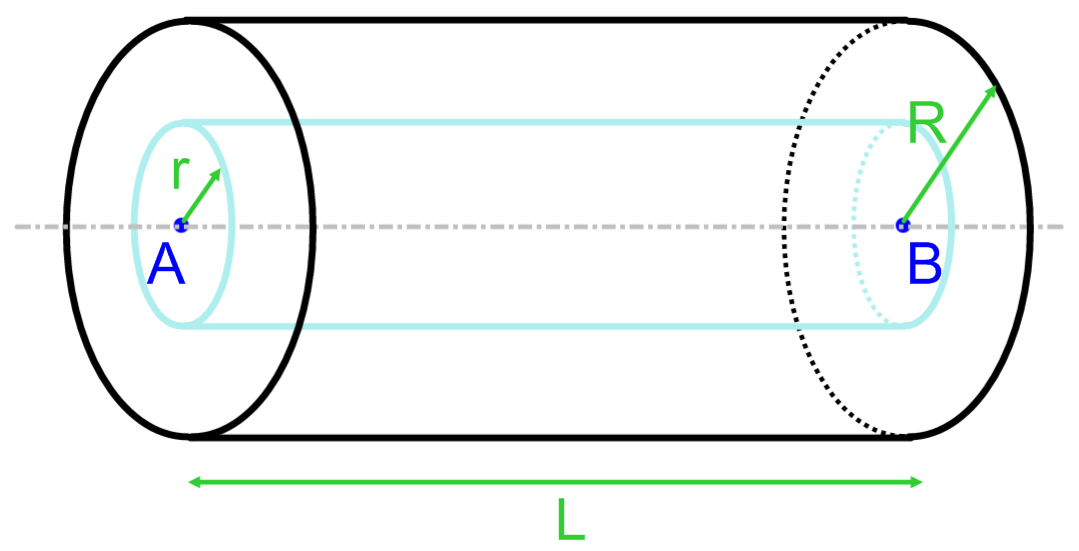
\includegraphics[width=0.5\paperwidth]{slike/slika1.PNG}
\end{center}
\begin{itemize}
\item zbog razlike tlakova na bazama valjka javlja se sila iznosa
\[
F_{\Delta p}=p_{_{A}}S_{_{A}}-p_{_{B}}S_{_{B}}=(p_{_{A}}-p_{_{B}})S_{baze}=\Delta p\:\pi r^{2}
\]
\item zbog viskoznog trenja javlja se posmično naprezanje $\tau$ na plaštu
valjka te je iznos ukupne sile viskoznog trenja
\[
F_{vt}=\tau\,S_{pla\check{s}ta}=\tau\:2\pi rL
\]
\end{itemize}
\end{frame}

\begin{frame}{Laminarno tečenje kroz nagnutu cijev}

\begin{center}
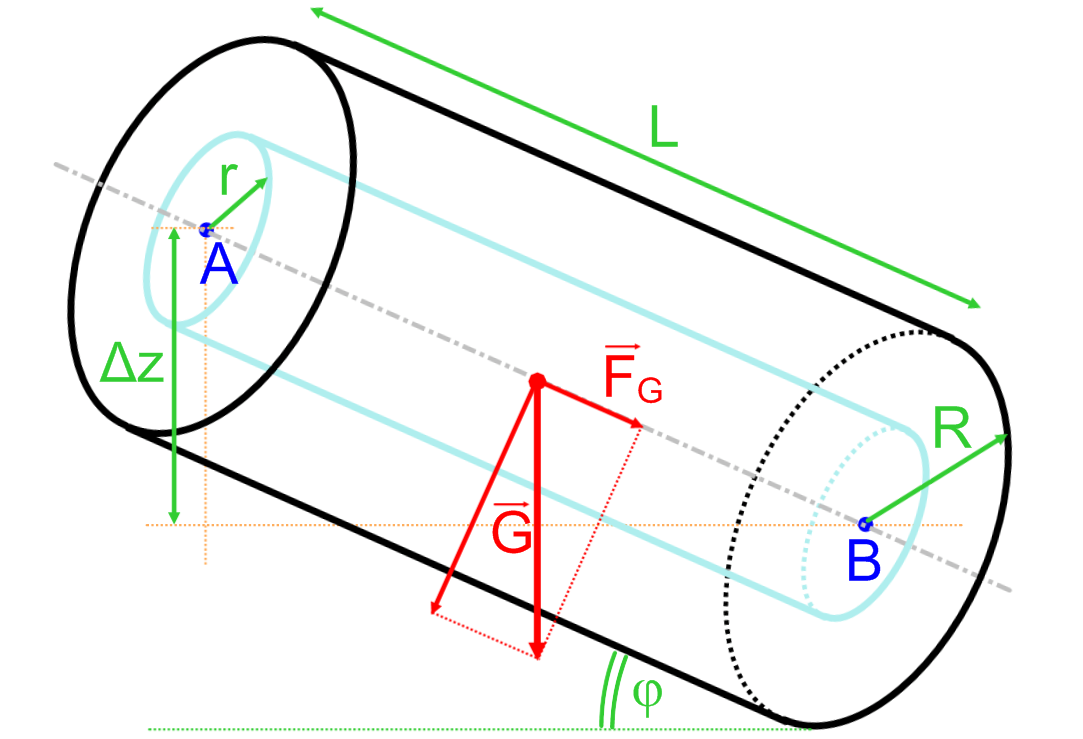
\includegraphics[width=0.5\paperwidth]{slike/slika2.PNG}
\par\end{center}
\begin{itemize}
\item duž osi cijevi javlja se i treća sila --- komponenta sile teže koja
djeluje na cilindrični element tekućine
\[
F_{G}=G\sin\varphi=mg\sin\varphi=\rho Vg\sin\varphi=\rho\pi r^{2}Lg\sin\varphi
\]
\end{itemize}
\end{frame}

\begin{frame}{Kod jednolikog tečenja sile su u ravnoteži}

\begin{itemize}
\item sinus kuta $\varphi$ može se izraziti kao omjer razlike geodetskih
visina točaka A i B na krajevima cijevi i duljine segmenta cijevi
\[
\sin\varphi=\frac{z_{_{A}}-z_{_{B}}}{L}=\frac{\Delta z}{L}
\]
pa je projekcija sile teže duž osi cijevi
\[
F_{G}=\rho\pi r^{2}Lg\frac{\Delta z}{L}=\rho g\Delta z\:\pi r^{2}
\]
\item kod jednolikog tečenja sve sile duž osi cijevi su u ravnoteži, a kako
je sila viskoznog trenja koja se opire tečenju suprotne orijentacije,
slijedi 
\[
F_{\Delta p}+F_{G}=F_{vt}\quad\Rightarrow\quad\Delta p\:\pi r^{2}+\rho g\Delta z\:\pi r^{2}=\tau2\pi rL
\]
\end{itemize}
\end{frame}

\begin{frame}{Ukupna razlika tlakova}

\begin{itemize}
\item ponovo dobivamo da je ovisnost posmičnog naprezanja $\tau$ o $r$
linearna kao što je bilo i kod horizontalne cijevi
\[
\tau(r)=\frac{1}{2}\frac{\Delta p+\rho g\Delta z}{L}r=\frac{1}{2}\frac{\widehat{\Delta p}}{L}r
\]
\item međutim, u nazivniku je suma hidrauličkog i hidrostatičkog tlaka 
\[
\widehat{\Delta p}\equiv\Delta p+\rho g\Delta z
\]
 što predstavlja ukupnu razliku tlakova između točaka A i B
\item daljnji postupak rješavanja je isti kao i kod horizontalne cijevi,
a rezultati su ekvivalentni, osim što se umjesto $\Delta p$ uvrštava
ukupna razlika tlakova $\widehat{\Delta p}$
\end{itemize}
\end{frame}

\begin{frame}{Ovisnost brzine o $r$}

\begin{itemize}
\item najprije izjednačimo izraze za posmično naprezanje
\[
\tau=-\mu\frac{dv}{dr}=\frac{1}{2}\frac{\widehat{\Delta p}}{L}r
\]
\item pa razdvajamo (separiramo) varijable
\[
dv=-\frac{\widehat{\Delta p}}{2\mu L}rdr
\]
\item i ovisnost brzine o $r$ dobivamo integriranjem
\[
v(r)=-\frac{\widehat{\Delta p}}{2\mu L}\int rdr=-\frac{\widehat{\Delta p}}{2\mu L}\frac{r^{2}}{2}+C=-\frac{\widehat{\Delta p}}{4\mu L}r^{2}+C
\]
\end{itemize}
\end{frame}

\begin{frame}{Parabolična raspodjela brzina}

\begin{itemize}
\item konstanta integracije $C$ određuje se iz uvjeta $v(R)=0$ (\emph{``no-slip
condition}'') i ponovo dobivamo paraboličnu raspodjelu brzina
\[
v(r)=v_{0}\left(1-\frac{r^{2}}{R^{2}}\right)
\]
samo što je maksimalna brzina $v(r=0)=v_{0}$ ovisna o ukupnoj razlici
tlakova $\widehat{\Delta p}$
\[
v_{0}=\frac{\widehat{\Delta p}}{4\mu L}R^{2}
\]
\item srednja brzina opet je $\bar{v}=v_{0}/2$ pa je protok
\[
Q=\bar{v}S=\frac{v_{0}}{2}\pi R^{2}=\frac{\pi}{8}\frac{\widehat{\Delta p}}{\mu L}R^{4}=\frac{\pi}{128}\frac{\widehat{\Delta p}}{\mu L}D^{4}
\]
a to je dobro nam poznati \alert{Hagen-Poiseuilleov zakon}
\end{itemize}
\end{frame}

\begin{frame}{Hagen-Poiseuilleov zakon}

\begin{itemize}
\item ako okrenemo Hagen-Poiseuilleov zakon
\[
\widehat{\Delta p}=\frac{128}{\pi}\frac{\mu L}{D^{4}}Q=\frac{128}{\pi}\frac{\mu L}{D^{4}}\frac{v_{0}}{2}\pi\frac{D^{2}}{4}=16\frac{\mu L}{D^{2}}v_{0}
\]
\item to možemo kombinirati s
\[
\widehat{\Delta p}=\Delta p+\rho g\Delta z=p_{_{A}}-p_{_{B}}+\rho g(z_{_{A}}-z_{_{B}})
\]
pa preslagivanjem članova 
\[
p_{_{A}}+\rho gz_{_{A}}=p_{_{B}}+\rho gz_{_{B}}+16\frac{\mu L}{D^{2}}v_{0}
\]
dobijemo nešto što počinje ličiti na Bernoullijevu jednadžbu
\end{itemize}
\end{frame}

\begin{frame}{Modificirana Bernoullijeva jednadžba}

\begin{itemize}
\item na strujnici koja prolazi središtem cijevi ($r = 0$) vrijedi $v_{_{A}}=v_{_{B}}=v_{_{0}}$
pa možemo dodati i dinamičke tlakove koji nedostaju
\[
p_{_{A}}+\rho gz_{_{A}}+\frac{1}{2}\rho v_{_{A}}^{2}=p_{_{B}}+\rho gz_{_{B}}+\frac{1}{2}\rho v_{_{B}}^{2}+16\frac{\mu L}{D^{2}}v_{0}
\]
i sličnost s Bernoullijevom jednadžbom je potpuna
\item međutim, s desne strane pojavio se još jedan dodatni član koji opisuje
\textbf{gubitak specifične energije zbog viskoznog trenja}
\end{itemize}
\begin{alertblock}{}
Dakle, da bi se opisalo tečenje realne (stvarne, viskozne) tekućine
nužno je modificirati Bernoullijevu jednadžbu!
\end{alertblock}
\end{frame}

\section{Energijska jednadžba}
\begin{frame}{Ponavljanje: Ograničenja u primjeni Bernoullijeve jednadžbe}

\textbf{Bernoullijeva jednadžba} je izvedena uz sljedeća ograničenja:
\begin{itemize}
\item neviskozno tečenje (opisuje tečenje idealne, neviskozne tekućine)
--- zanemareno je viskozno trenje!
\item stacionarno tečenje
\item tečenje nestlačivog fluida (zapravo nije problem --- tekućine su
praktički nestlačive)
\item tečenje duž strujnice
\end{itemize}
\begin{alertblock}{}
\textcolor{blue}{\large{}\alert{Energijska jednadžba}} je modificirana
Bernoullijeva jednadžba koja opisuje stacionarno tečenje stvarne, viskozne tekućine u
cjevovodu. Povezuje dva presjeka cijevi i služi za proračun cjevovoda.
\end{alertblock}
\end{frame}

\begin{frame}{Energijska jednadžba}

\begin{alertblock}{Energijska jednadžba}
\[
\frac{p_{{\scriptscriptstyle A}}}{\rho g}+z_{{\scriptscriptstyle A}}+\alpha_{{\scriptscriptstyle A}}\frac{\bar{v}_{{\scriptscriptstyle A}}^{2}}{2g}+h_{P}-h_{T}=\frac{p_{{\scriptscriptstyle B}}}{\rho g}+z_{{\scriptscriptstyle B}}+\alpha_{{\scriptscriptstyle B}}\frac{\bar{v}_{{\scriptscriptstyle B}}^{2}}{2g}+h_{F}
\]
\end{alertblock}
\begin{description}
\item [{$h_{P}$}] -- visina dobave pumpe ($m$)
\item [{$h_{T}$}] -- pad visine na turbini ($m$)
\item [{$\bar{v}_{A},\bar{v}_{B}$}] -- srednje brzine na presjecima cijevi
A i B ($ms^{-1}$)
\item [{$\alpha_{_{A}},\alpha_{_{B}}$}] -- Coriolisovi koeficijenti (bezdimenzionalni)
\item [{$h_{F}$}] -- ukupna visina gubitaka, zbroj svih linijskih i lokalnih
gubitaka u cjevovodu ($m$)
\end{description}
\end{frame}

\begin{frame}{Linijski i lokalni gubici}

\begin{itemize}
\item \alert{linijski gubici} su gubici u cijevima i računaju se pomoću
Darcy-Weisbachove formule
\[
h_{f}=\lambda\frac{L}{D}\frac{\bar{v}^{2}}{2g}
\]
\item \alert{lokalni gubici} tlaka javljaju se u manjoj ili većoj mjeri
na suženjima, proširenjima, koljenima, ventilima i svim drugim elementima
cjevovoda i proporcionalni su kvadratu srednje brzine, tj. brzinskoj
visini 
\[
h_{fm}=K_{L}\frac{\bar{v}^{2}}{2g}
\]
pri čemu je $K_{L}$ \textbf{lokalni koeficijent otpora} karakterističan
za pojedini element cjevovoda
\end{itemize}
\end{frame}

\begin{frame}{Ukupna visina gubitaka}

\begin{block}{}
\textbf{Ukupna visina gubitaka u cjevovodu} je zbroj svih linijskih
i lokalnih gubitaka u cjevovodu
\[
h_{F}=\sum_{i=1}^{N_{C}}h_{f,i}+\sum_{j=1}^{N_{L}}h_{fm,j}
\]
\end{block}
pri čemu je
\begin{description}
\item [{$N_{C}$}] -- broj cijevi koje su serijski spojene u cjevovod
\item [{$N_{L}$}] -- broj elemenata u cjevovodu na kojima dolazi do lokalnih
gubitaka
\end{description}
\end{frame}

\begin{frame}{Specifična kinetička energija na presjeku cijevi}

\begin{itemize}
\item u Bernoullijevoj jednadžbi brzinska visina predstavlja specifičnu
kinetičku energiju po jedinici težine tekućine koja prolazi kroz jednu
određenu točku
\item u energijskoj jednadžbi više se ne promatra jedna točka na strujnici
već čitav presjek cijevi
\item detaljni proračun pokazuje da za srednji protok specifične kinetičke
energije kroz presjek cijevi vrijedi
\[
\bar{\rho}_{Ek}\geq\frac{1}{2}\rho\bar{v}^{2}
\]
\item znak jednakosti $\bar{\rho}_{Ek}=\frac{1}{2}\rho\bar{v}^{2}$ realiziran
je samo za specijalni slučaj kad je brzina na cijelom presjeku cijevi
ista, tj. kada je $v=konst.=\bar{v}$
\end{itemize}
\end{frame}

\begin{frame}{Coriolisov koeficijent}

\begin{itemize}
\item kada brzine na presjeku cijevi znatno odstupaju od srednje brzine
$\bar{v}$ tada i $\bar{\rho}_{Ek}$ postaje znatno veća od $\frac{1}{2}\rho\bar{v}^{2}$
pa je to potrebno korigirati odgovarajućim koeficijentom koji se označava
s $\alpha$, a naziva \alert{Coriolisov koeficijent}
\item iz poznate parabolične raspodjele brzina kod laminarnog
tečenja može se izračunati da je za laminarno tečenje $\alpha=2$
\item međutim, kod turbulentnog tečenja tekućina se (osim tankog rubnog
sloja) zbog transverzalnih komponenti brzine stalno miješa pa se gotovo
sva tekućina na presjeku cijevi giba brzinom koja je približno jednaka
srednjoj brzini --- u tom slučaju Coriolisov koeficijent je samo
malo veći od jedan
\end{itemize}
\begin{block}{}

\begin{itemize}
\item za turbulentno tečenje najčešće se uzima $\alpha=1$
\end{itemize}
\end{block}
\end{frame}

\begin{frame}{Primjena energijske jednadžbe: proračun cjevovoda}

\begin{alertblock}{Energijska jednadžba služi za proračun cjevovoda}
\begin{itemize}
\item to je modificirana Bernoullijeva jednadžba za tečenje stvarne, viskozne
tekućine u cjevovodu
\item uobičajeno je da je u visinskom obliku
\item disipacija mehaničke energije zbog viskoznog trenja uzima se u obzir
kroz visinu linijskih i lokalnih gubitaka 
\item za razliku od Bernoullijeve jednadžbe koja je relacija između dvije
točke na strujnici, energijska jednadžba je relacija između dva presjeka
cijevi duž cjevovoda
\item opisuje stacionarno tečenje
\end{itemize}
\end{alertblock}
\end{frame}

\begin{frame}{Proračun cjevovoda: vrste problema}

Kod proračuna cjevovoda tipično se javljaju tri vrste problema:
\begin{itemize}
\item poznati su geometrija i elementi cjevovoda: treba izračunati gubitke
\item poznati su geometrija i elementi cjevovoda: treba izračunati protok
(ili, ekvivalentno, srednju brzinu tečenja na nekom presjeku cjevovoda) 
\item tipičan inženjerski problem: treba odabrati i dimenzionirati elemente
cjevovoda kako bi se dobio željeni protok (poželjno je i da se to
realizira uz minimalne troškove)
\end{itemize}
Drugi i treći tip problema su nešto složeniji --- do rješenje se
dolazi iteracijom.
\end{frame}

\section{Tečenje u cijevima proizvoljnog presjeka}
\begin{frame}{Tečenje u cijevima proizvoljnog presjeka}

\begin{itemize}
\item cijev kružnog presjeka moguće je opisati jednim parametrom: to je
polumjer cijevi $R$
\item pokazalo se da je cijevi proizvoljnog presjeka također moguće opisati
jednim parametrom, takozvanim \textit{hidrauličkim polumjerom $R_{h}$}
\end{itemize}
\begin{alertblock}{Definicija: Hidraulički polumjer}
\[
R_{h}\equiv\frac{S}{O}\equiv\frac{povr\check{s}ina\:presjeka}{omo\check{c}eni\:obod}
\]
\end{alertblock}
\begin{itemize}
\item definicija je univerzalna, vrijedi i za cijevi koje nisu u potpunosti
ispunjene tekućinom, kao i za sve vrste otvorenih kanala i korita,
pa se zato spominje\emph{ omočeni} obod
\end{itemize}
\end{frame}

\begin{frame}{Primjer 1: Cijev kvadratičnog presjeka}

\begin{center}
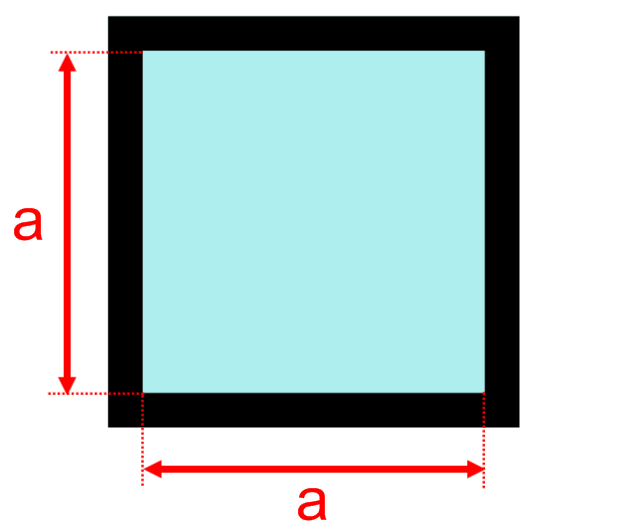
\includegraphics[width=0.3\paperwidth]{slike/slika3.PNG}
\par\end{center}
\begin{example}
{Cijev kvadratičnog presjeka duljine stranica $a$}

\[
R_{h}=\frac{povr\check{s}ina\:kvadrata}{opseg\:kvadrata}=\frac{a^{2}}{4a}=\frac{a}{4}
\]

\end{example}

\end{frame}

\begin{frame}{Primjer 2: Cijev pravokutnog presjeka}

\begin{center}
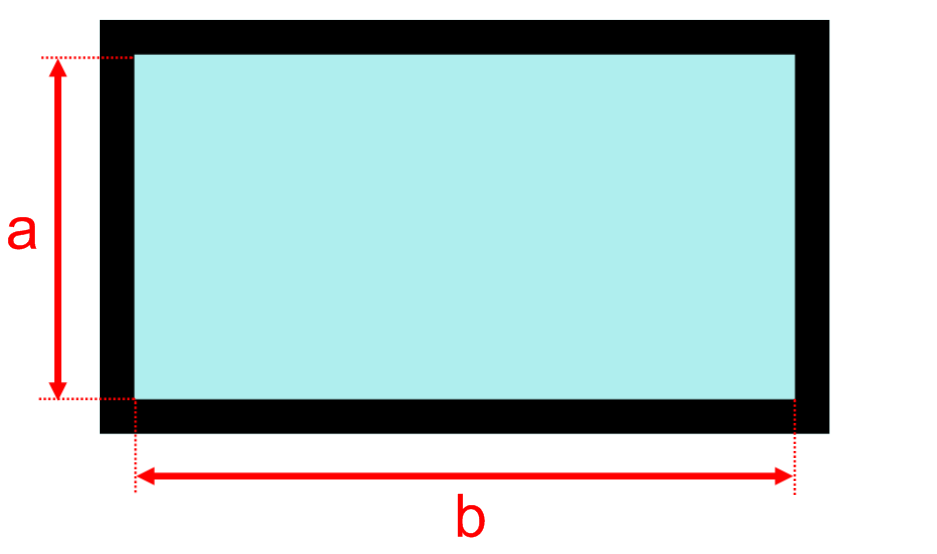
\includegraphics[width=0.45\paperwidth]{slike/slika4.PNG}
\par\end{center}
\begin{example}
{Cijev pravokutnog presjeka duljina stranica $a$ i $b$}

\[
R_{h}=\frac{povr\check{s}ina\:pravokutnika}{opseg\:pravokutnika}=\frac{a\,b}{2\,(a+b)}
\]

\end{example}

\end{frame}

\begin{frame}{Primjer 3: Cijev kružnog presjeka}

\begin{center}
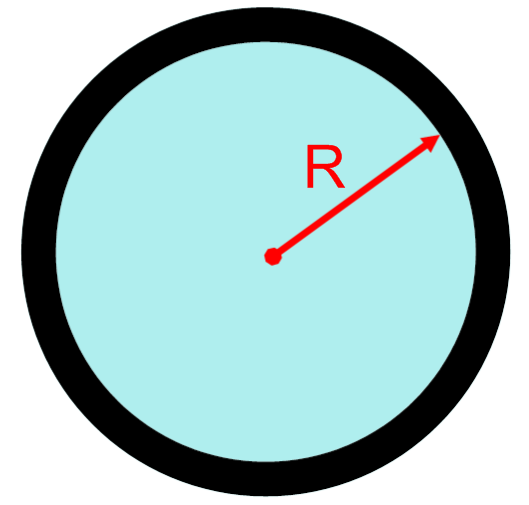
\includegraphics[width=0.3\paperwidth]{slike/slika5.PNG}
\par\end{center}
\begin{example}
{Cijev kružnog presjeka polumjera $R$}

\[
R_{h}=\frac{povr\check{s}ina\:kruga}{opseg\:kru\check{z}nice}=\frac{\pi R^{2}}{2\pi R}=\frac{R}{2}
\]

\end{example}

\end{frame}

\begin{frame}{Hidraulički promjer}

\begin{itemize}
\item nelogičan rezultat da je hidraulički polumjer $R_{h}$ cijevi kružnog
presjeka pola od stvarnog polumjera cijevi $R$ potencijalno komplicira
stvari pa se to popravlja sljedećom definicijom
\end{itemize}
\begin{alertblock}{Definicija: Hidraulički promjer}
\[
D_{h}\equiv4R_{h}
\]
\end{alertblock}
\begin{itemize}
\item tako je hidraulički promjer za cijev kružnog presjeka $D_{h}=4R_{h}=4R/2=2R$,
tj. $D_{h}=D$ pa je moguće poopćiti definicije i formule koje sadrže
promjer cijevi $D$ zamjenom $D\rightarrow D_{h}$, tj. umjesto promjera
$D$ uvrštava se hidraulički promjer $D_{h}$
\end{itemize}
\end{frame}

\begin{frame}{Poopćenja za cijev proizvoljnog presjeka}

\begin{block}{Reynoldsov broj}
\[
\mathrm{Re}\equiv\frac{\rho\bar{v}D_{h}}{\mu}=\frac{\bar{v}D_{h}}{\nu}
\]
\end{block}
\begin{itemize}
\item isto vrijedi i za Darcy-Weisbachovu formulu: promjer kružne cijevi
$D$ zamijeni se hidrauličkim promjerom $D_{h}$ i dobije se visina
gubitaka pri tečenju kroz cijev proizvoljnog presjeka
\end{itemize}
\begin{block}{Darcy-Weisbachova formula za cijev proizvoljnog presjeka}
\[
h_{f}=\lambda\frac{L}{D_{h}}\frac{\bar{v}^{2}}{2g}
\]
\end{block}
\end{frame}

\end{document}
